\documentclass[12pt,a4paper]{article}
\usepackage[utf8]{inputenc}
\usepackage[T1]{fontenc}
\usepackage{amsmath}
\usepackage{amsthm}
\usepackage{amssymb}
\usepackage{graphicx}
\usepackage{enumitem}
\usepackage{newunicodechar}
\usepackage{algpseudocode}
\usepackage{algorithm}
\newunicodechar{≤}{\ensuremath{\leq}}

\title{Algoritmer og Datastrukturer (NDAA04010U) Ugeopgave 4}
\author{Københavns Universitet}
\date{2025}

\begin{document}
\maketitle

\section{Dynamisk programmering}

En stigende delsekvens af en tabel A, der indeholder heltal A[1], \ldots, A[n], er en delmængde af indekser $1 \leq i_1 < i_2 < \cdots < i_k \leq n$ således at A[$i_1$] < A[$i_2$] < $\cdots$ < A[$i_k$]. Længden af delsekvensen er antal indekser, k. En ikke-aftagende delsekvens defineres på samme måde bortset fra at kravet er A[$i_1$] $\leq$ A[$i_2$] $\leq \cdots \leq$ A[$i_k$]. Betragt følgende funktion, i pseudo-kode notationen fra CLRS, hvor input A er en tabel af heltal.

\begin{verbatim}
MaximumMystery(A, n)
1 let r[1...n] be a new array
2 r[1] = 1
3 for j = 2 to n
4     q = 1
5     for i = 1 to j - 1
6         if not A[j] < A[i]
7             q = max(q, r[i] + 1)
8     r[j] = q
9 return max{1≤j≤n} r[j]
\end{verbatim}

Hvad beregner proceduren MaximumMystery? Vælg præcis ét svar og beskriv hvordan du kom frem til det. Formulér en invariant for den ydre løkke som en del af dit svar.

\begin{enumerate}
\item Indekserne i en længste stigende delsekvens.
\item Indekserne i en længste ikke-aftagende delsekvens.
\item Længden af en længste stigende delsekvens.
\item Længden af en længste ikke-aftagende delsekvens. \textbf{Korrekt}
\end{enumerate}

vi kan se dette, da for hvert index j tæller vi antallet af elementer, før j som er mindre end eller lig elementet i position A[j]. 

for den ydre lykke har vi den invariant at 
for $j \geq 2$ gælder at $r[j]$ er længden af den længste ikke-aftagende delsekvens der ender ved j, og 
for alle $i < j$ hvor $A[i] \leq A[j]$ gælder $r[j] \geq r[i] + 1$

\section{Huffman koder}

Vi betragter algoritmen til konstruktion af Huffman koder i CLRS sektion 15.3.

a) Tegn Huffman træet som algoritmen beregner for alfabetet C = \{a, b, c, d, e\} med frekvenser $f_a = 5$, $f_b = 8$, $f_c = 3$, $f_d = 7$, $f_e = 1$. Det er ikke nødvendigt at angive labels (0 og 1) på kanterne, men angiv frekvenser i blade såvel som indre knuder.


% Her kan du indsætte et billede af Huffman træet
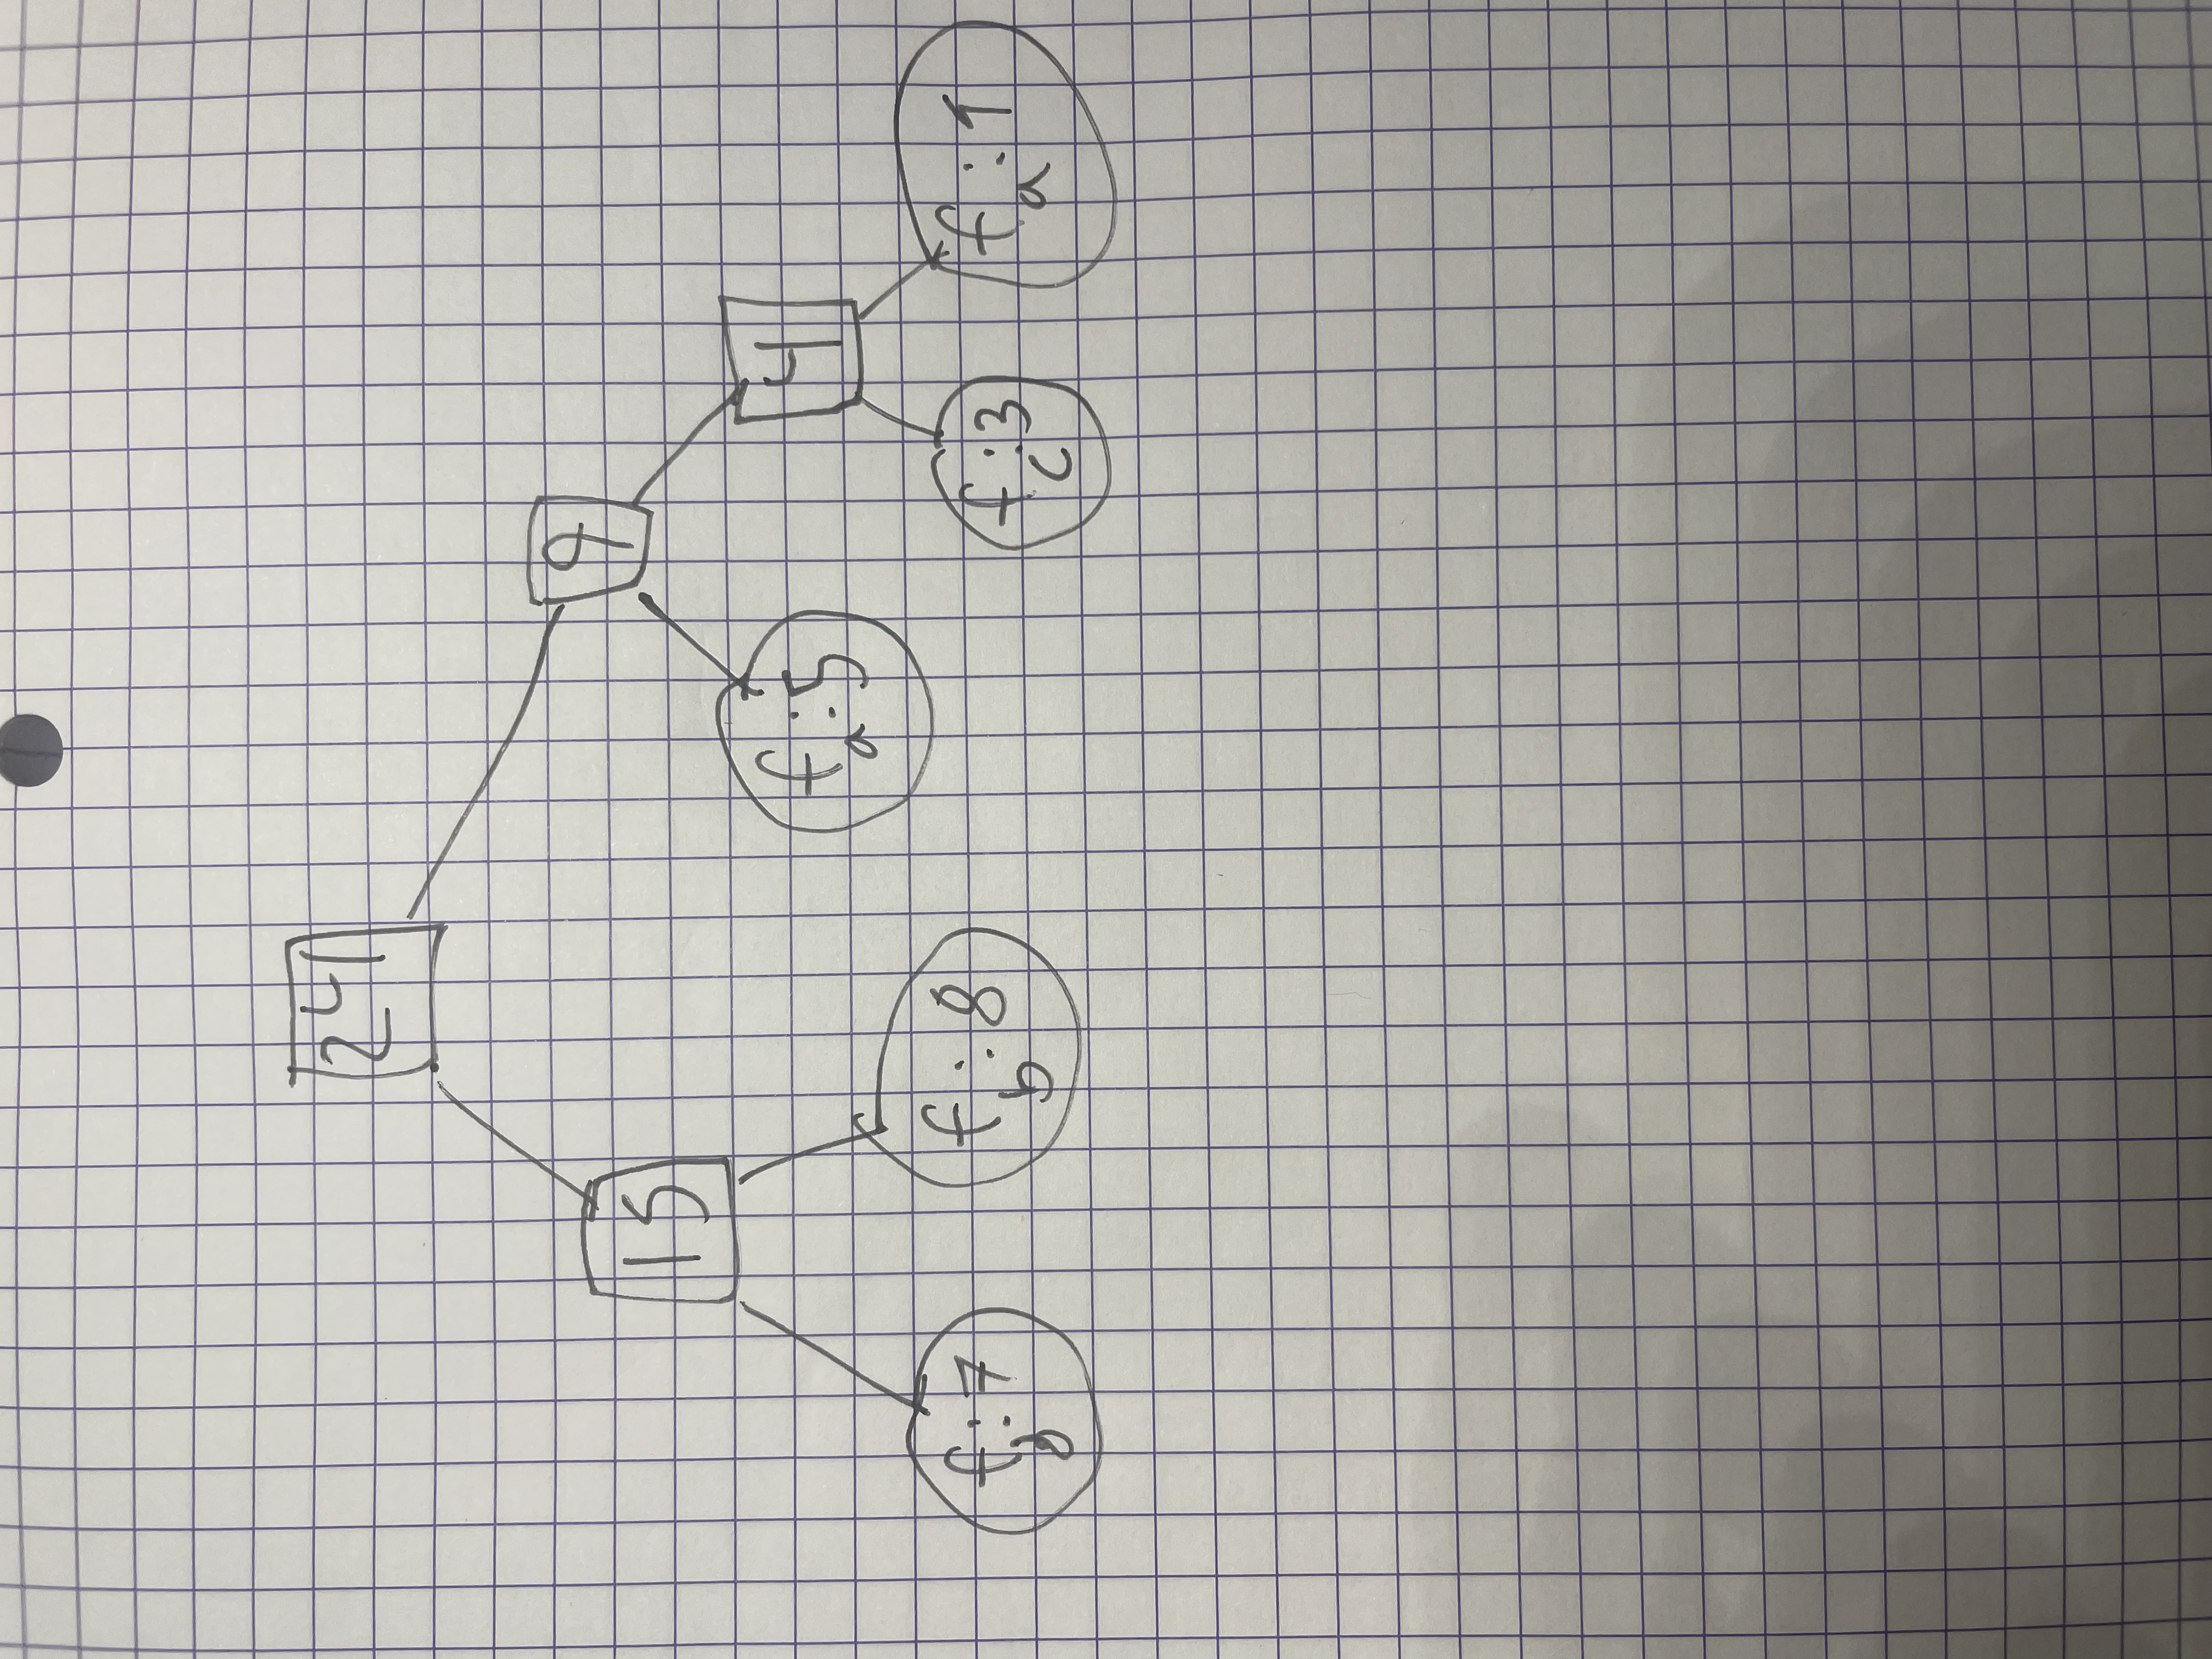
\includegraphics[width=0.7\textwidth]{IMG_9968.jpeg}

\section{Mere dynamisk programmering}

Vi et givet en liste $x_0, x_1, \ldots, x_n$ med n positive heltal. Betragt følgende rekursive definition af værdier $m_{i,j}$, hvor $1 \leq i \leq j \leq n$:

\[m_{i,j} = \begin{cases} 
1 & \text{hvis } i = j\\
\max\{m_{i,k} + m_{k+1,j} + x_{i-1}x_kx_j \mid i \leq k < j\} & \text{hvis } i < j
\end{cases}\]

En rekursiv algoritme der direkte følger rekursionsligningen, uden at gemme beregnede værdier, bruger tid $O(t_{i,j})$ til at beregne $m_{i,j}$, hvor

\[t_{i,j} = \begin{cases}
1 & \text{hvis } i = j\\
1 + \sum_{k=i}^{j-1} t_{i,k} + t_{k+1,j} & \text{hvis } i < j
\end{cases}\]

a) Argumentér for at $t_{i,j} \geq 2^{j-i+1} - 1$. Brug gerne induktion i $\ell = j - i$.

Vi viser dette ved induktion i $\ell = j - i$.

\begin{enumerate}
    \item \textbf{Base Case} $\ell = 0$
    without loss of generality antag $j=i=1$
    $t_{1,1} = 1$ da $j=i$
    dvs $t_{1,1} = 1 \geq 2^{1-1+1} = 1$
    \item \textbf{Induktions Skridt}
    vi har nu følgende IH $t_{i,j} \geq 2^{\ell+1} - 1$ hvor $\ell = j-i$ 

    vi undersøger nu $\ell = (j+1) - i$

    \[t_{i, j+1} = 1 + \sum_{k=i}^{(j+1)-1} t_{i,k} + t_{k+1,(j+1)} =
    \underbrace{\left(1 +  \sum_{k=i}^{j-1} t_{i,k} + t_{k+1,j}\right)}_{t_{i,j}} + t_{i,j} + t_{j, j+1} = 2t_{i, j} + t_{j, j+1}\]

    vi har nu
    \[
    t_{i, j+1} = 2t_{i, j} + t_{j, j+1} \underbrace{\geq}_{t_{j, j+1} \geq 1} 2t_{i, j} + 1 \underbrace{\geq}_{IH} 2(2^{(j-i)+1} - 1) + 1
    \]
    \[
    = 2 \cdot 2^{(j-i)+1} - 2 + 1 =  2^{((j+1)-i)+1} - 1
    \]
    
    og vi er færdige.
\end{enumerate}

b) Forklar, gerne med pseudokode, hvordan dynamisk programmering kan bruges til effektivt at beregne $m_{i,j}$ for alle $1 \leq i \leq j \leq n$. Analysér plads og køretid for algoritmen, i store-O notation, som funktion af n.

vi foreslår følgende algoritme

\begin{algorithm}
\caption{Dynamisk programmering til beregning af $m_{i,j}$}
\begin{algorithmic}
\Function{BeregneM}{$x_0, x_1, \ldots, x_n$}
    \State Opret en $n \times n$ tabel $M$ hvor $M[i,j]$ vil indeholde værdien af $m_{i,j}$
    
    \For{$i = 1$ \textbf{to} $n$}
        \State $M[i,i] \gets 1$ \Comment{Basistilfælde: $m_{i,i} = 1$}
    \EndFor
    
    \For{$\ell = 1$ \textbf{to} $n-1$} \Comment{$\ell$ er længden af intervallet}
        \For{$i = 1$ \textbf{to} $n-\ell$}
            \State $j \gets i + \ell$
            \State $M[i,j] \gets -\infty$ \Comment{Initialisér til en meget lav værdi}
            \For{$k = i$ \textbf{to} $j-1$}
                \State $q \gets M[i,k] + M[k+1,j] + x_{i-1} \cdot x_k \cdot x_j$
                \If{$q > M[i,j]$}
                    \State $M[i,j] \gets q$
                \EndIf
            \EndFor
        \EndFor
    \EndFor
    
    \State \Return $M[1,n]$ \Comment{Returnerer den optimale værdi $m_{1,n}$}
\EndFunction
\end{algorithmic}
\end{algorithm}

Algoritmen bruger dynamisk programmering til at beregne alle værdier af $m_{i,j}$ for $1 \leq i \leq j \leq n$. Vi beregner værdierne i rækkefølge af stigende intervallængde $\ell = j-i$.

\textbf{Tidskompleksitet:} Algoritmen har tre loops

\[
\sum_{\ell=1}^{n-1}\sum_{i=1}^{n-\ell}\sum_{k=i}^{i+\ell-1} = O(n^3)
\]

\textbf{Pladskompleksitet:} Vi bruger en $n \times n$ tabel til at gemme alle værdier af $m_{i,j}$, så pladskompleksiteten er $O(n^2)$.

Sammenlignet med den rekursive algoritme, som bruger eksponentiel tid $\Omega(2^n)$ som vist i del a), giver den dynamiske programmerings-tilgang en væsentlig forbedring med polynomiel tidskompleksitet.


\section{Grådige algoritmer}

Vi betragter igen MaxProduct problemet fra Ugeopgave 2:

Givet en liste af tal $x_1, \ldots, x_n \in \mathbb{R}$ (kan være både positive og negative), find en delmængde $I^* \subseteq \{1, \ldots, n\}$ hvor produktet $\prod_{i\in I^*} x_i$ er så stort som muligt, dvs. for alle mængder $I \subseteq \{1, \ldots, n\}$ skal gælde at $\prod_{i\in I} x_i \leq \prod_{i\in I^*} x_i$.

\textbf{Eksempel.} På input $x_1 = -4$, $x_2 = -0.5$, $x_3 = 0.5$, $x_4 = 0.5$, $x_5 = 1.5$, $x_6 = 6$ kan vi vælge $I = \{5, 6\}$ og få et produkt på $1.5 \cdot 6 = 9$, men et bedre valg er $I = \{1, 2, 5, 6\}$ som giver produktet $(-4) \cdot (-0.5) \cdot 1.5 \cdot 6 = 18$. Den tomme mængde $I = \emptyset$ giver per definition $\prod_{i\in\emptyset} x_i = 1$.

Et mulig tilgang til at løse MaxProdukt er at grådigt føje elementer til I, ét ad gangen. Antag at input er sorteret således at $x_1 \leq x_2 \leq \cdots \leq x_n$.

a) Argumentér for at for en optimal løsning $I^*$ vil der altid vil være et lige antal elementer i mængden $I^*_- = \{i \in I^* \mid x_i < 0\}$, dvs. $|I^*_-|$ er deleligt med 2.

Hvis $|I^*_-|$ er ulige, betyder det at produktet af elementerne i sættet $\prod_{i \in I^*_-} x_i < 0$

Da $I^*_- \subseteq I^*$ har vi altså $\prod_{i \in I^*_-} x_i \cdot \prod_{i \in I^* \setminus I^*_-} x_i < 0$

b) Foreslå en effektiv algoritme til at finde en optimal løsning $I^*$. Argumentér for korrekthed og køretid. Der lægges vægt på, at argumentationen er klar og koncis.

\begin{algorithm}
\caption{MaxProduct}
\begin{algorithmic}[1]
    \Function{MaxProduct}{$x_1, x_2, \ldots, x_n$}
        \State $I^* \gets \emptyset$ \Comment{Initialisér den optimale mængde}
        \State $I_{pos} \gets \emptyset$ \Comment{Initialisér mængde for positive tal}
        \State $I_{neg} \gets \emptyset$ \Comment{Initialisér mængde for negative tal}
        
        \State Sortér input således at $x_1 \leq x_2 \leq \cdots \leq x_n$
        
        \For{$i \gets 1$ \textbf{to} $n$}
            \If{$x_i \geq 1$}
                \State $I_{pos} \gets I_{pos} \cup \{i\}$
            \ElsIf{$x_i \leq -1$}
                \State $I_{neg} \gets I_{neg} \cup \{i\}$
            \EndIf
        \EndFor
        
        \State $I^* \gets I^* \cup I_{pos}$ \Comment{Tilføj alle positive tal $\geq 1$ til løsningen}
        
        \If{$|I_{neg}|$ er lige}
            \State $I^* \gets I^* \cup I_{neg}$ \Comment{Tilføj alle negative tal $\leq -1$ hvis der er et lige antal}
        \Else
            \State Sortér $I_{neg}$ efter stigende absolut værdi: $|x_{i_1}| \leq |x_{i_2}| \leq \ldots$
            \State $I^* \gets I^* \cup I_{neg} \setminus \{i_1\}$ \Comment{Fjern det negative tal med mindste absolutte værdi}
        \EndIf
        
        \State \Return $I^*$
    \EndFunction
\end{algorithmic}
\end{algorithm}
Algoritmen er korrekt af følgende grunde:

\begin{enumerate}
    \item Vi maksimerer produktet ved at inkludere alle tal, der bidrager positivt:
    \begin{enumerate}
        \item Alle positive tal $\geq 1$ inkluderes, da de altid øger produktet.
        \item Negative tal $\leq -1$ inkluderes parvis, da produktet af to negative tal er positivt.
    \end{enumerate}
    
    \item Vi håndterer negative tal optimalt:
    \begin{enumerate}
        \item Hvis der er et lige antal negative tal $\leq -1$, inkluderer vi dem alle, hvilket giver et positivt bidrag.
        \item Hvis der er et ulige antal, fjerner vi det med mindste absolutte værdi for at sikre et positivt samlet produkt.
    \end{enumerate}
    
    \item Vi udelader alle tal i intervallet $(-1, 1)$, da multiplikation med disse ville reducere produktets absolutte værdi.
    
    \item Algoritmen garanterer det maksimale produkt ved systematisk at vælge den optimale delmængde baseret på tallenes fortegn og absolutte værdier.
\end{enumerate}

Køretidsanalyse:
\begin{enumerate}
    \item Sortering af input: $O(n \log n)$
    \item Gennemløb af arrayet for at identificere positive og negative tal: $O(n)$
    \item Sortering af negative tal efter absolut værdi (i værste tilfælde): $O(n \log n)$
    \item Øvrige operationer (union af mængder, etc.): $O(n)$
\end{enumerate}

Den samlede køretid er derfor $O(n \log n)$, domineret af sorteringsoperationerne.

\end{document}
